% !TEX root =  paper.tex
\section{Method}

\begin{figure}[t]
	\centering
	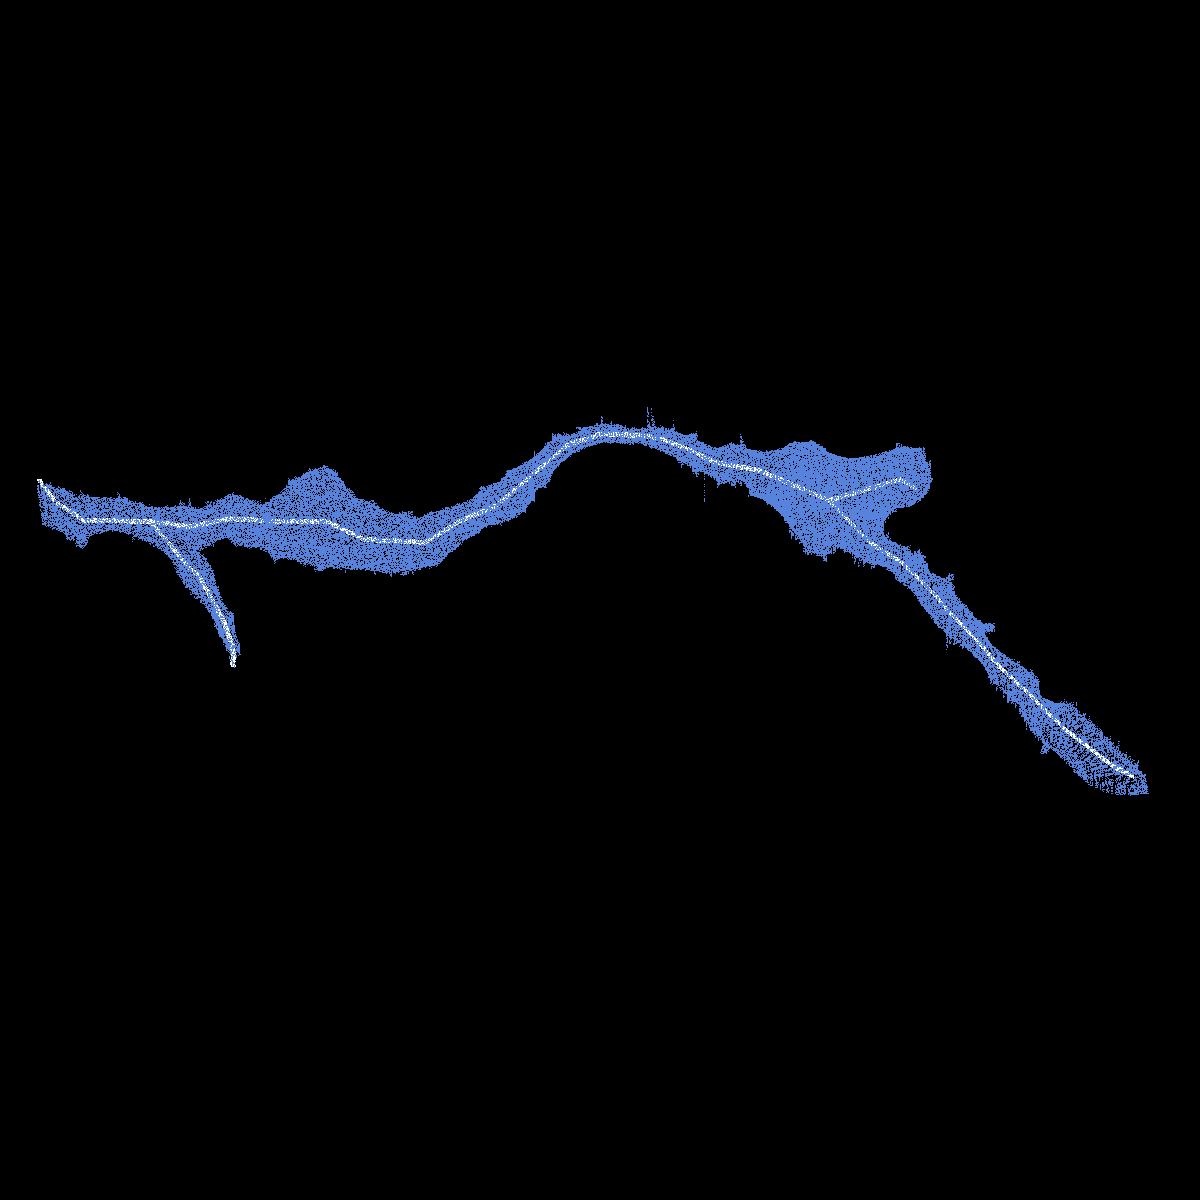
\includegraphics[width=0.92\linewidth]{./figures/skeleton1.png}
	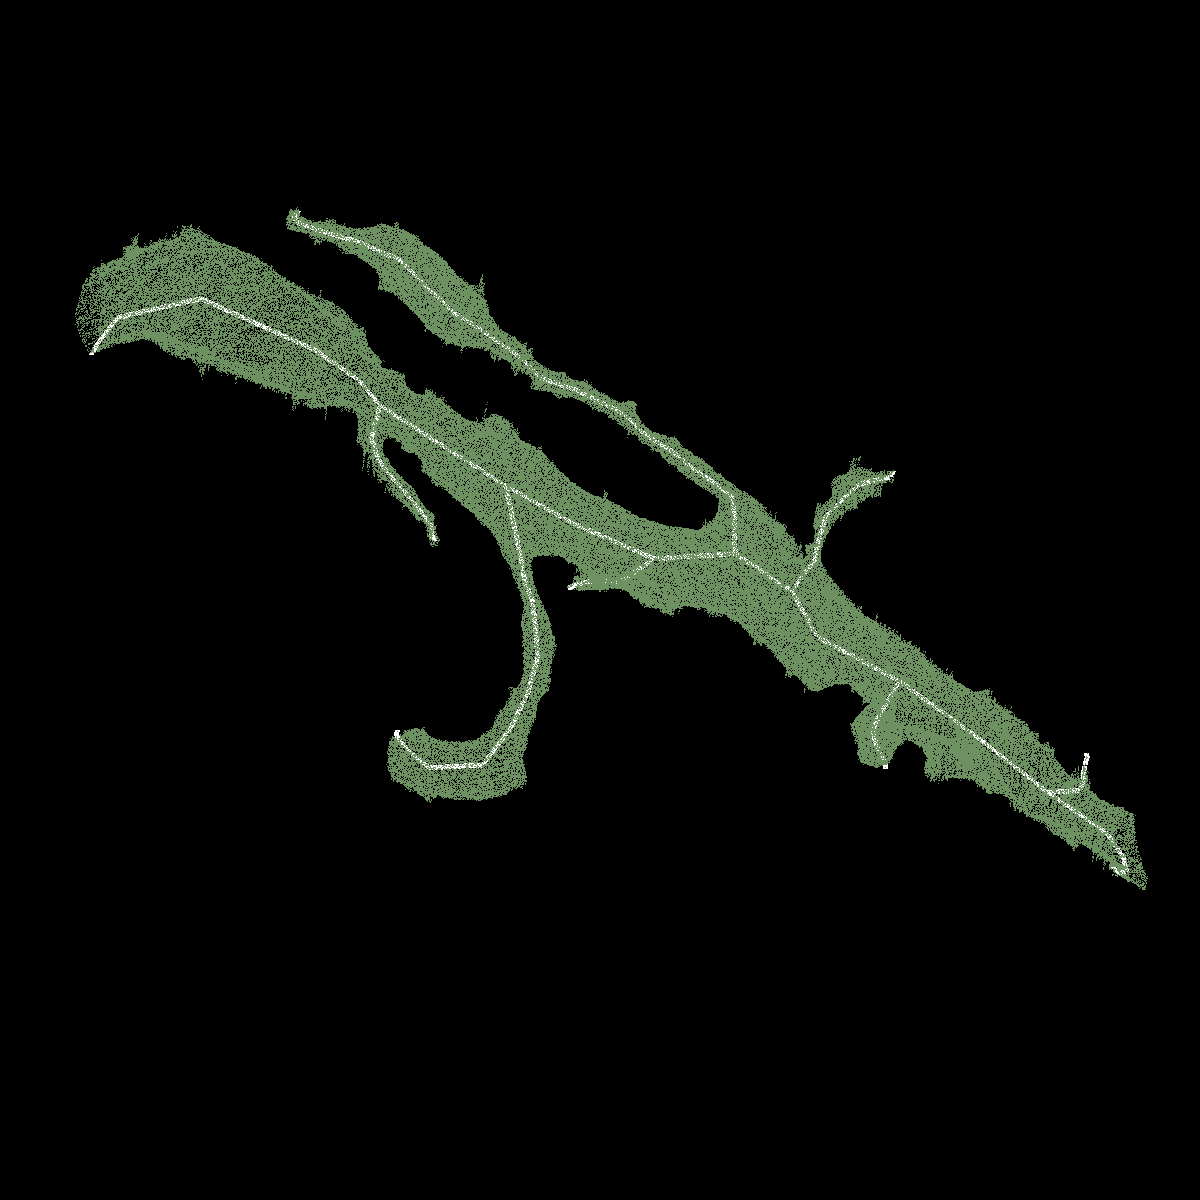
\includegraphics[width=0.92\linewidth]{./figures/skeleton2.png}
	\caption{Example skeletons (in white) extracted from segments (blue and green) using the TEASER algorithm.}
	\label{fig:skeletonization}
\end{figure}

There are two types of errors that can occur in connectomics segmentation.
The first, called a split error, occurs when there are two segments that should have been merged. The second, called a merge error, happens when one segment should be split into two. Generally, it is much more difficult to correct merge errors than to correct split errors~\cite{parag2015properties}, which is why most reconstruction approaches are tuned towards over-segmentation with many more split than merge errors. Our method takes as input over-segmentations of EM image volumes generated by state-of-the-art connectomics reconstruction pieplines (Sec.~\ref{sec:neuroproof}). Our goal is to identify locations of split errors and merge the corresponding segments automatically.

From the input segmentation we generate a graph $G$ with nodes $N$ and edges $E$ with non-negative edge weights $w_e$. The nodes correspond to label segments from the segmentation with edges between segments considered for merging. Ideally, our graph has edges corresponding to all of the segments that were erroneously split. To compute this graph we generate a skeleton for every segment in the pixel-based segmentation. The skeleton is a simplified representation of the overall shape of the neurons. From this skeleton we  identify potential merge locations and produce the corresponding edges for the graph. To find actual merges we run a classification CNN to generate edge weights that correspond to probabilites of merging. We then use a multicut heuristic to generate a partition on the graph where nodes in the same partition are assigned the same output label in the improved segmentation. We will now discuss the three major components to our framework (graph creation, edge probabilities, and graph partitioning) in more detail.

\subsection{Graph Creation}
\label{sec:skeletonization}

%We generate nodes $N$ and edges $E$ to apply a graph-based optimization strategy for segmentation.
%In addition, these edges receive non-negative weights.

\subsubsection{Node Generation}

The simplest node generation strategy creates one node for every unique segment label in the input volume. However, some of the millions of labels in the volume correspond to very small structures that are likely the result of segmentation errors. This typically happens in regions with noisy image data such that pixel-based methods could not generate the correct segments. It is difficult to extract useful shape features from these segments because of their small, and often random, shape. We prune these nodes from the graph by removing all segments with fewer than a threshold of $t_{seg}$ voxels. We use $t_{seg} = 20,000$ voxels, which removed on average XX\% \hp{add} of the segments in our  datasets (Sec.~\ref{sec:dataset}).

\subsubsection{Edge Generation}

A typical approach to generating edges produces an edge between all adjacent segments. Two segments $l_1$ and $l_2$ are considered adjacent if there is a pair of adjacent voxels where one has label $l_1$ and the other has label $l_2$.
For example, pixel-based agglomeration methods such as NeuroProof~\cite{} and GALA~\cite{} \hp{add refs} consider all pairs of adjacent segments for merging.
However, this method produces too many edges in the graph for graph-based optimization approaches. We identify a smaller number of pairs of segments to consider as graph edges using the following algorithm.

First, we extract a skeleton from each segment using the TEASER algorithm~\cite{sato2000teasar,zhao2014automatic}. Fig.~\ref{fig:skeletonization} shows an example of two extracted skeletons (in white) of two segments from the label volume. These skeletons consist of a sequence of \textit{joints}, i.e., locations that are a local maximum distance from the segment boundary, with line segments connecting successive joints. We prune the joints that are within $t_{jnt} = 50$ voxels of each other to reduce unnecessary branching. For the purposes of our algorithm, joints that have only one connected neighbor are referred to as \textit{endpoints}. Many of the segments that are erroneously split have nearby endpoints  (Fig.~\ref{fig:merge_candidates}). We will make use of this fact to merge segments with the following two-pass heuristic.

In the first pass, we iterate over all endpoints $e$ belonging to a segment $S$ and create a set of segments $\mathbb{S}_e^\prime$ that includes all labels that are within $t_{low}$ voxels from $e$. Elements of $\mathbb{S}_e^\prime$ are candidates for merging. However, this first pass often leads to too many candidates, requiring an additional pass for further pruning. In the second pass, we consider all of the segments in $\mathbb{S}_e^\prime$ for every endpoint $e$. If a segment $S^\prime \in \mathbb{S}_e^\prime$ has an endpoint within $t_{high}$ voxels of $e$, the segment $S$ and $S^\prime$ are considered for merging. We store the midpoints between the two endpoints as the center of the potential merges in the set $\mathbb{S}_c$.

\begin{figure}[t]
	\centering
	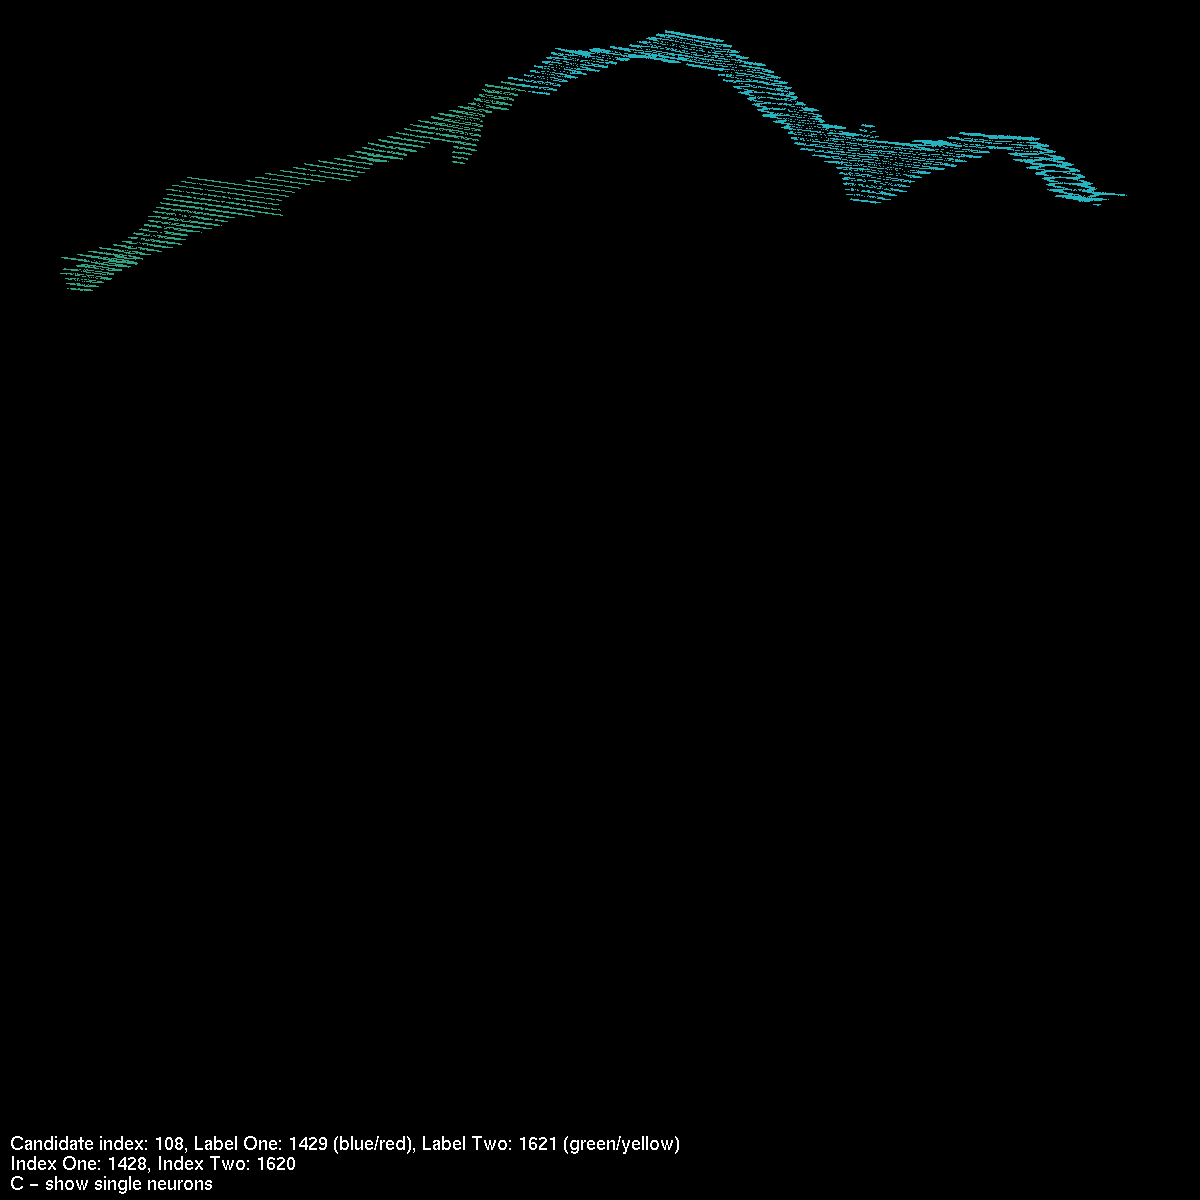
\includegraphics[width=0.92\linewidth]{./figures/split_error1.png}
	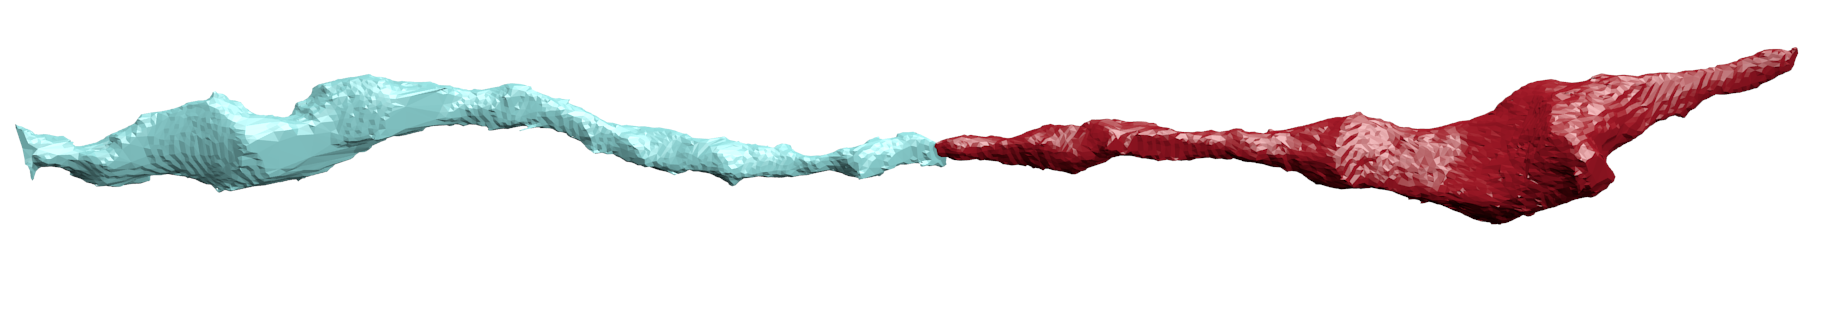
\includegraphics[width=0.92\linewidth]{./figures/split_error2.png}
	\caption{Two erroneously split segments. \hp{split in top figure impossible to see - use brighter colors. both figures are too dark - increase brightness of segments}}
	\label{fig:merge_candidates}
\end{figure}

\subsection{Edge Probabilities}

Our non-negative edge weights $w_e$ correspond to probabilities that two endpoints $e$ in $\mathbb{S}_c$ belong to the same neuron and should be merged. \hp{check} To compute these probabilities we train a 3D CNN classifier using the oversegmentation input volume and corresponding manually labeled ground truth data (Sec.~\ref{sec:dataset}).

\subsubsection{Classifier Input}

We extract a cubic region of interest around each endpoints $e$ in $\mathbb{S}_c$ as input to the CNN. These regions of interest provide the local information for the neural network to predict which neighboring segments belong to the same neuron. The CNN receives three input channels for every voxel in the region of interest around segments $l_1$ and $l_2$. The input in all of the channels is in the range $\{-0.5, 0.5\}$. The first channel is $0.5$ only if the corresponding voxel has label $l_1$. The second channel is $0.5$ only if the corresponding voxel has label $l_2$. The third channel is $0.5$ if the corresponding voxel is either $l_1$ or $l_2$.

\subsubsection{Network Architecture \& Training}

Fig.~\ref{fig:architecture} provides an overview of our CNN architecture. Similar to Chatfield et al.~\cite{chatfield2014return} it consists of three layers of double convolutions followed by a max pooling step. The first max pooling layer is anisotropic with pooling only in the $x$ and $y$ dimensions. The output of this final pooling step is flattened into a 1D vector that is input into two fully connected layers. The final layer produces probabilities with a sigmoid activation function~\cite{funahashi1989approximate}. All of the other activation functions are LeakyReLU~\cite{maas2013rectifier}.

We use a stochastic gradient descent optimizer with Nesterov's accelerated gradient~\cite{nesterov1983method} for training. We employ dropouts of $0.2$ after every pooling layer and the first dense layer, and a dropout of $0.5$ after the final dense layer to prevent overfitting. We discuss all other network parameters in Sec.~\ref{sec:network-parameters}.

\begin{figure*}[t]
	\centering
	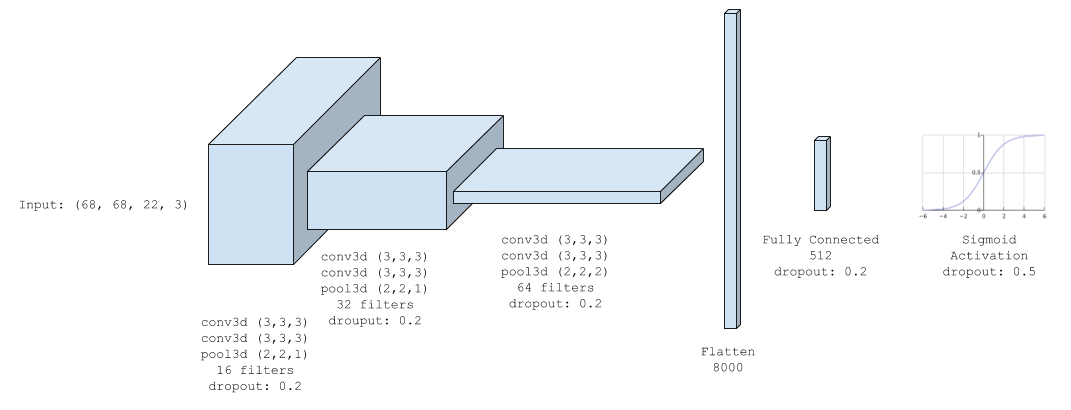
\includegraphics[width=0.95\linewidth]{figures/architecture.png}
	\caption{The architecture for our classification CNN uses double convolutions followed by max pooling. The number of filters doubles each layer, with a final fully connected layer and sigmoid activation function.}
	\label{fig:architecture}
\end{figure*}

\subsection{Graph Partitioning}

After constructing the 3D graph we apply graph-based partitioning to compute the final segmentation. Using graph partitioning from the top down allows us to apply biological constraints on the output. Neuroscientists know that neuronal connectivity graphs in the brain are acyclic (i.e., the graphs have a genus of zero). We enforce this constraint by finding a multicut partition of the graph that generates a \textit{forest} of nodes. A forest is a partitioning of a graph into a set of trees where no segment has a cycle. To solve this constraing multicut problem we use the method by Keuper et al.~\cite{keuper2015efficient} that produces a feasible solution by greedy additive edge contraction. Adding additional constraints and improving the graph partition algorithm are areas for future work.
